%--------------------------------------------------------------------------------
%
%--------------------------------------------------------------------------------
\unnumberedChapter{The Runtime Library (RtLib)}

The Runtime Library (\texttt{RtLib}) is the software foundation of every LCS node. It forms the interface between the application firmware and the underlying hardware module and provides the common services required by every node.

Rather than manipulating hardware directly, application firmware interacts almost exclusively with the runtime library. RtLib manages node configuration, communication on the Layout Control Bus, event processing, port management, and the storage of persistent configuration data. The library also provides convenient methods for sending messages to other nodes and allows the application firmware to register callback functions that react to messages, events, and timer expirations.

One of the primary design goals of RtLib is to shield the firmware programmer from the internal implementation of the runtime. Instead of directly accessing internal data structures, firmware interacts with the node through a well-defined set of library functions. This approach keeps application firmware independent of the runtime implementation while allowing the library to transparently manage synchronization, validation, communication, and persistent storage.

The following sections introduce the runtime data model before describing how application firmware accesses node data and services.

%--------------------------------------------------------------------------------
\unnumberedSection{Runtime Data Model}

The runtime organizes all node information into several memory areas called \textbf{maps}. Each map groups together a particular category of runtime data, such as node configuration, port information, event subscriptions, or user data.

Some maps exist only in volatile memory, referred to as \texttt{MEM}, while others have both a volatile and a non-volatile representation. The non-volatile storage, referred to as \texttt{NVM}, preserves configuration information across power cycles.

During node startup, every persistent map is initialized by copying its contents from the corresponding NVM map into MEM. Once initialization has completed, the runtime operates exclusively on the MEM version for maximum performance. Whenever persistent changes are required, the runtime synchronizes the modified data back to the corresponding NVM map.

Maps without an NVM counterpart contain purely transient runtime information. They are initialized from default values compiled into the runtime library whenever the node starts.

\begin{center}
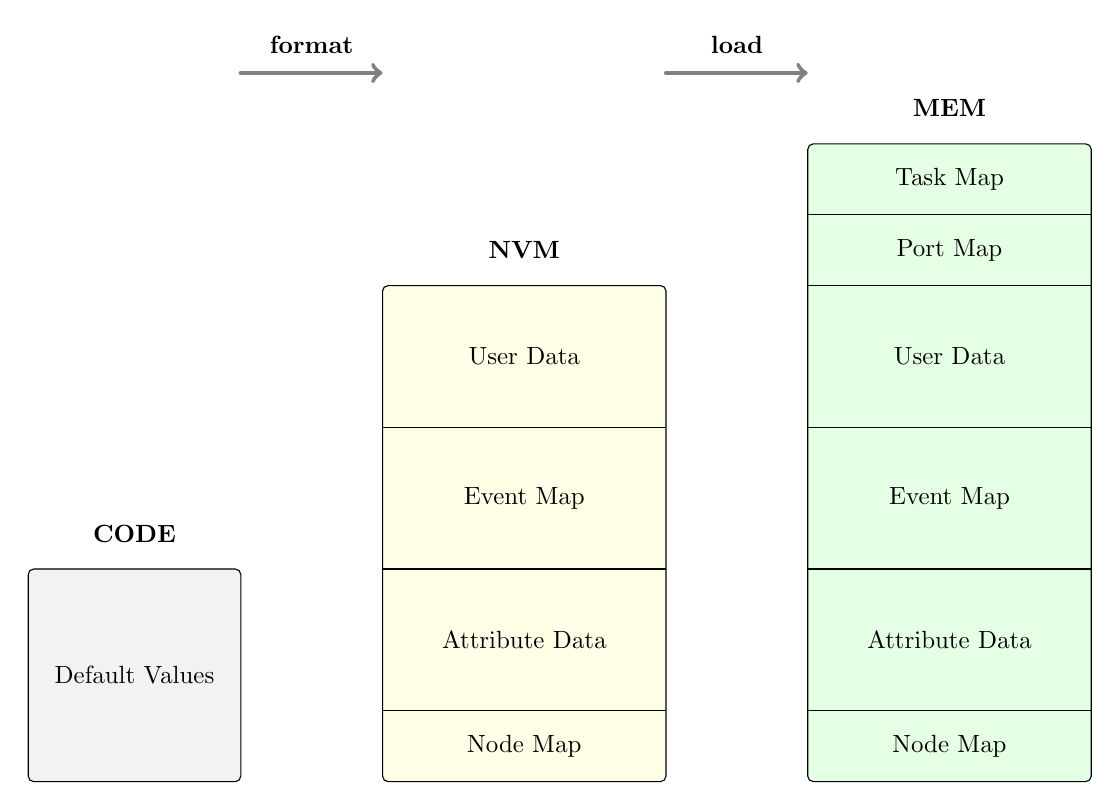
\begin{tikzpicture}[scale=0.9, transform shape]

     % flow
     \node at (4,10.4) {\textbf{format}};
     \draw[->, ultra thick, gray, line cap=round] (3,10) -- (5,10);

     \node at (10,10.4) {\textbf{load}};
     \draw[->, ultra thick, gray, line cap=round] (9,10) -- (11,10);

     % rectangles
     \draw[rounded corners=2pt, fill=gray!10] (0,0) rectangle (3,3);
     \draw[rounded corners=2pt, fill=yellow!10] (5,0) rectangle (9,7);
     \draw[rounded corners=2pt, fill=green!10] (11,0) rectangle (15,9);

     % code
     \node at (1.5,3.5) {\textbf{CODE}};
     \node at (1.5,1.5) {Default Values};

     % NVM
     \node at (7,7.5) {\textbf{NVM}};
     \node at (7,0.5) {Node Map};
     \draw (5,1)--(9,1);

     \node at (7,2) {Attribute Data};
     \draw (5,3)--(9,3);

     \node at (7,4) {Event Map};
     \draw (5,5)--(9,5);

     \node at (7,6) {User Data};

     % MEM
     \node at (13,9.5) {\textbf{MEM}};
     \node at (13,0.5) {Node Map};
     \draw (11,1)--(15,1);

     \node at (13,2) {Attribute Data};
     \draw (11,3)--(15,3);

     \node at (13,4) {Event Map};
     \draw (11,5)--(15,5);

     \node at (13,6) {User Data};
     \draw (11,7)--(15,7);

     \node at (13,7.5) {Port Map};
     \draw (11,8)--(15,8);

     \node at (13,8.5) {Task Map};

\end{tikzpicture}
\end{center}
\FloatBarrier

The separation between MEM and NVM serves two important purposes. First, it allows the runtime to operate entirely from RAM, providing efficient access to frequently used data structures. Second, it avoids unnecessary writes to non-volatile memory, whose write endurance is limited compared to RAM. Only data that must survive a restart is synchronized back to NVM.

%--------------------------------------------------------------------------------
\unnumberedSubSection{Fixed Map Sizes}

Each runtime map has a predefined size. For example, the Port Map always contains one entry for every physical port supported by the node, while the Event Map reserves space for a fixed maximum number of event subscriptions.

An alternative design would have allowed each node to configure the size of its individual maps. RtLib deliberately avoids this approach in favor of a fixed memory layout.

There are several reasons for this design decision.

First, node initialization requires no memory configuration. Every node shares the same internal memory layout, simplifying both firmware development and maintenance.

Second, the required memory is modest compared to the resources available on modern controller hardware. A generously configured node supporting 128 node attributes, eight ports each with 128 port attributes, an event table containing 1024 entries, and additional runtime data requires only about 9~KBytes of storage. Even a modest 32~KByte EEPROM therefore leaves considerable room for application-specific user data, while controllers such as the RP2040 provide more than enough RAM for the runtime structures.

Finally, a fixed layout greatly simplifies runtime initialization. Persistent maps can be restored directly from NVM without reconstructing variable-sized data structures or performing dynamic memory allocation. This keeps startup deterministic and avoids unnecessary implementation complexity.

The result is a runtime system with a simple, predictable memory layout that requires no configuration while consuming only a small fraction of the available hardware resources.

%--------------------------------------------------------------------------------
\unnumberedSection{Runtime Maps}

The runtime maintains several maps, each serving a specific purpose. Together they describe the complete operational state of an LCS node.

Although these maps are internal runtime data structures, they are not manipulated directly by application firmware. Instead, the runtime library provides controlled access through its programming interface. This allows the library to maintain consistency, synchronize persistent data, and perform internal bookkeeping transparently to the firmware programmer.

The following sections briefly introduce each runtime map.

%--------------------------------------------------------------------------------
\unnumberedSubSection{Node Map}

The Node Map contains the internal configuration and status information of the node itself. It is the central runtime data structure from which the library obtains all information required to manage the remaining maps.

Typical information stored in the Node Map includes the Node ID, CAN ID, library version, runtime options, pointers to the remaining runtime maps, and additional internal state information required by the library.

The Node Map exists both in MEM and in NVM. During startup, the runtime initializes the MEM version from the corresponding NVM map. Once the node is operational, all accesses are performed on the MEM copy. Whenever persistent configuration changes are required, the modified data is synchronized back to NVM.

Application firmware never accesses the Node Map directly. Instead, the runtime exposes selected information through the standard GET and SET interface described later in this chapter. This keeps the internal implementation independent from the external programming interface and allows the runtime to evolve without affecting application firmware.

%--------------------------------------------------------------------------------
\unnumberedSubSection{Port Map}

The Port Map contains the current runtime state of every physical port supported by the node. It consists of one Port Map entry for each port.

Each entry stores information describing both the configuration and the current operating state of the corresponding port. This includes configuration flags, the current event being processed, pending actions, delayed event execution, callback information, and other runtime state required by the event dispatcher.

Unlike the Node Map, the Port Map is purely a runtime data structure and therefore exists only in MEM. It is recreated whenever the node starts and does not require persistent storage.

The runtime continuously updates the Port Map while processing incoming events and executing application callbacks. For this reason, application firmware should regard the Port Map as runtime-owned data and use the provided library functions whenever port information needs to be queried or modified.

%--------------------------------------------------------------------------------
\unnumberedSubSection{Event Map}

The Event Map defines the set of Layout Control Bus events that are of interest to the node.

Each Event Map entry contains an Event ID together with a port mask identifying the ports that should receive this event whenever it is observed on the Layout Control Bus.

The runtime maintains two different representations of the Event Map.

The persistent representation stored in NVM consists of a simple array of Event Map entries. This representation is compact and well suited for configuration tools that sequentially read or update the event database.

During startup, the runtime constructs a second representation in MEM. This runtime representation is organized as a hash table, allowing very fast lookup of incoming Event IDs during normal operation.

The separation between persistent storage and runtime representation allows the event dispatcher to perform efficient lookups without compromising the simplicity of the on-chip storage format.

The maximum number of Event Map entries is fixed at compile time. The current runtime library supports up to 512 event subscriptions.

Whenever the Event Map is modified, dedicated runtime services synchronize the MEM and NVM representations. Reading the Event Map is supported both during normal operation and while the node is in configuration mode. Creating or deleting Event Map entries, however, is only permitted while the node is operating in configuration mode.

%--------------------------------------------------------------------------------
\unnumberedSubSection{Periodic Task Map}

Most embedded applications perform recurring activities. Typical examples include polling sensors, updating displays, generating flashing patterns, supervising communication timeouts, or performing regular housekeeping functions.

Rather than requiring every application to implement its own timing loop, RtLib provides a simple periodic task scheduler.

Application firmware registers a callback function together with the desired execution interval. The runtime stores this information in the Periodic Task Map and invokes the callback whenever the requested interval has elapsed.

This approach considerably simplifies firmware development while allowing the runtime to retain complete control over the main execution loop. Internal runtime services and application callbacks therefore share the same scheduling mechanism, ensuring deterministic execution without requiring the application to manage timers explicitly.

The Periodic Task Map contains only transient runtime information and therefore exists exclusively in MEM.


%--------------------------------------------------------------------------------
\unnumberedSection{Attributes and Item IDs}

Besides its internal runtime maps, every LCS node exposes a configurable set of attributes. These attributes represent the configuration and application data of the node and can be accessed both by the local application firmware and remotely through Layout Control Bus messages.

Conceptually, node attributes are similar to the Configuration Variables (CVs) used in DCC systems. However, RtLib considerably extends this concept. In addition to configurable attributes, the same programming interface also provides access to runtime variables and callable functions.

RtLib distinguishes between three categories of attributes.

\begin{itemize}
    \item \textbf{Node Attributes} describe properties of the node as a whole.
    \item \textbf{Port Attributes} belong to an individual port and typically describe its behaviour or configuration.
    \item \textbf{Global User Data} provides a large application-defined storage area whose size depends solely on the available non-volatile memory.
\end{itemize}

Node and port attributes are stored in NVM and copied into MEM during node startup. During normal operation, all accesses are performed on the MEM copy. Persistent storage is updated explicitly by synchronization requests or automatically while the node operates in configuration mode.

The Global User Data area occupies the remaining NVM after the runtime maps have been allocated. Consequently, its size depends on the storage available on the hardware module. For example, a node equipped with a 64~KByte EEPROM provides approximately 28,000 user-accessible data items after the runtime data has been reserved.

%--------------------------------------------------------------------------------
\unnumberedSubSection{Item IDs}

All information managed by RtLib is accessed through an \textbf{Item ID}. An Item ID is simply an integer that identifies either a runtime variable, an attribute, or a callable function.

Using a single addressing mechanism greatly simplifies both the runtime implementation and the programming interface. Rather than requiring different APIs for configuration data, runtime services, hardware channels, and application callbacks, RtLib uses Item IDs throughout.

The same Item ID may therefore represent different objects depending on the operation being performed.

\begin{itemize}
    \item For \textbf{GET} operations, an Item ID identifies a readable variable or attribute.
    \item For \textbf{SET} operations, an Item ID identifies a writable variable or attribute.
    \item For \textbf{REQ} operations, an Item ID invokes either a runtime service or an application-defined callback.
\end{itemize}

To simplify dispatching, the Item ID space is divided into several reserved ranges.

\begin{table}[!ht]
\begin{center}
\begin{tabularx}{0.9\textwidth}{|c|c|X|}
\hline
\textbf{Low} & \textbf{High} & \textbf{Purpose} \\
\hline
0 & 0 &
Reserved NIL Item.\\
\hline
1 & 63 &
Standard runtime items. Depending on the operation, these Item IDs either access standardized node and port variables or invoke built-in runtime services.\\
\hline
64 & 127 &
Channel Item IDs. GET, SET and REQ operations are dispatched directly to the corresponding hardware channel.\\
\hline
128 & 255 &
Application Item IDs. GET and SET operations access node or port attributes, while REQ operations invoke application-defined callback functions.\\
\hline
256 & NVM\_MAX &
Global User Data stored in the application-defined NVM area.\\
\hline
\end{tabularx}
\end{center}
\caption{Item ID ranges.}
\end{table}

\FloatBarrier

The first range is reserved entirely for the runtime library. These Item IDs provide standardized access to node information that is common to every LCS node, such as node properties, port status, and built-in runtime services.

The second range is dedicated to hardware channels. This allows the runtime to forward GET, SET and REQ operations directly to the responsible channel implementation without additional interpretation. The channel architecture is described in detail later in this book.

The third range is reserved for application firmware. GET and SET operations access the application's node and port attributes, whereas REQ operations invoke application-defined callback functions.

Finally, all Item IDs above 255 address the Global User Data area. This storage is entirely application-defined and can be used for arbitrary persistent information.

%--------------------------------------------------------------------------------
\unnumberedSubSection{Why Item IDs?}

The Item ID concept is one of the central architectural elements of RtLib.

First, it provides a uniform programming model. Application firmware, configuration tools, and remote nodes all use exactly the same addressing mechanism, regardless of whether they access a runtime variable, an attribute, a hardware channel, or an application-defined function.

Second, dispatching requests is extremely efficient. The runtime determines the destination of a request through a few simple range comparisons, avoiding complex lookup tables or dynamic registration mechanisms.

Third, the dedicated Channel Item range cleanly separates hardware-specific functionality from the core runtime library. New channel types can therefore be added without modifying the runtime itself.

Finally, the architecture remains highly extensible. While the lower Item ID ranges are standardized by RtLib, the application firmware is free to define its own attributes, callback functions, and persistent user data without conflicting with the runtime library.

The result is a compact, efficient, and flexible programming interface that remains consistent across all LCS nodes.

%--------------------------------------------------------------------------------
\unnumberedSection{Summary}

The runtime library organizes all persistent and runtime node data using maps. The
separation between non-volatile memory and memory storage is a fundamental design
concept.

At startup, the runtime initializes the memory representation of the node from the
non-volatile storage area. During normal operation, all access is performed through the
memory representation. Changes are synchronized back to non-volatile storage only when
required. This provides fast access during operation while avoiding unnecessary writes
to limited-lifetime non-volatile memory.

The main data structures introduced in this chapter are the node map, the port map and
the event map. The node map provides the central information about the node and its
associated data areas. The port map contains the configuration and operational data of
the node ports. The event map provides the association between incoming events and the
ports that react to them.

The non-volatile storage layout is tied to the runtime data structures. Changes to the
map organization, such as different numbers of entries or incompatible data structure
changes, require rebuilding the non-volatile area. Existing configuration data cannot be
automatically preserved across such structural changes and must be restored from an
external configuration source.

The runtime library provides a controlled access mechanism to this data through the
item-based programming model. Items provide a uniform way to access attributes,
runtime services and application-defined functionality.

The following chapter introduces the Runtime Library interfaces. It presents the
available functions and shows how firmware accesses the services provided by the
runtime layer.
